\documentclass[a4j]{jarticle}
\usepackage[dvipdfmx]{graphicx}
\usepackage{amssymb}
\usepackage{amsmath}
\usepackage{subfigure}
\newcommand{\argmax}{\mathop{\rm arg~min}\limits}

\begin{document}
\begin{table}[t]
\begin{center}
{\large 産業用モニタリングシステムにおける障害検知手法の提案}\\
令和 2 年 8 月 19 日\\
山本 航平
\end{center}
\end{table}

進捗報告
\begin{itemize}
\item 一日を通じた計測実験で見られる,低遅延帯が時間経過に伴い増加傾向を示す区間の抽出に取り組んでいます.
\end{itemize}

\section{低遅延帯の増加傾向}
一日を通じた計測データにおいて,小さな応答遅延の値が時間経過とともに増加していく傾向が部分的にみられる.ここでは FFT を用いて一部区間データ(6 月 23 日,6 月 24 日,6 月 25 日)におけるこの区間の時間的長さを調べた.
まず,この三つの区間データに対してそのまま FFT を用いた結果を図 \ref{fft} に示す.
\begin{figure}[tb]
\begin{center}
\subfigure[6 月 23 日]{
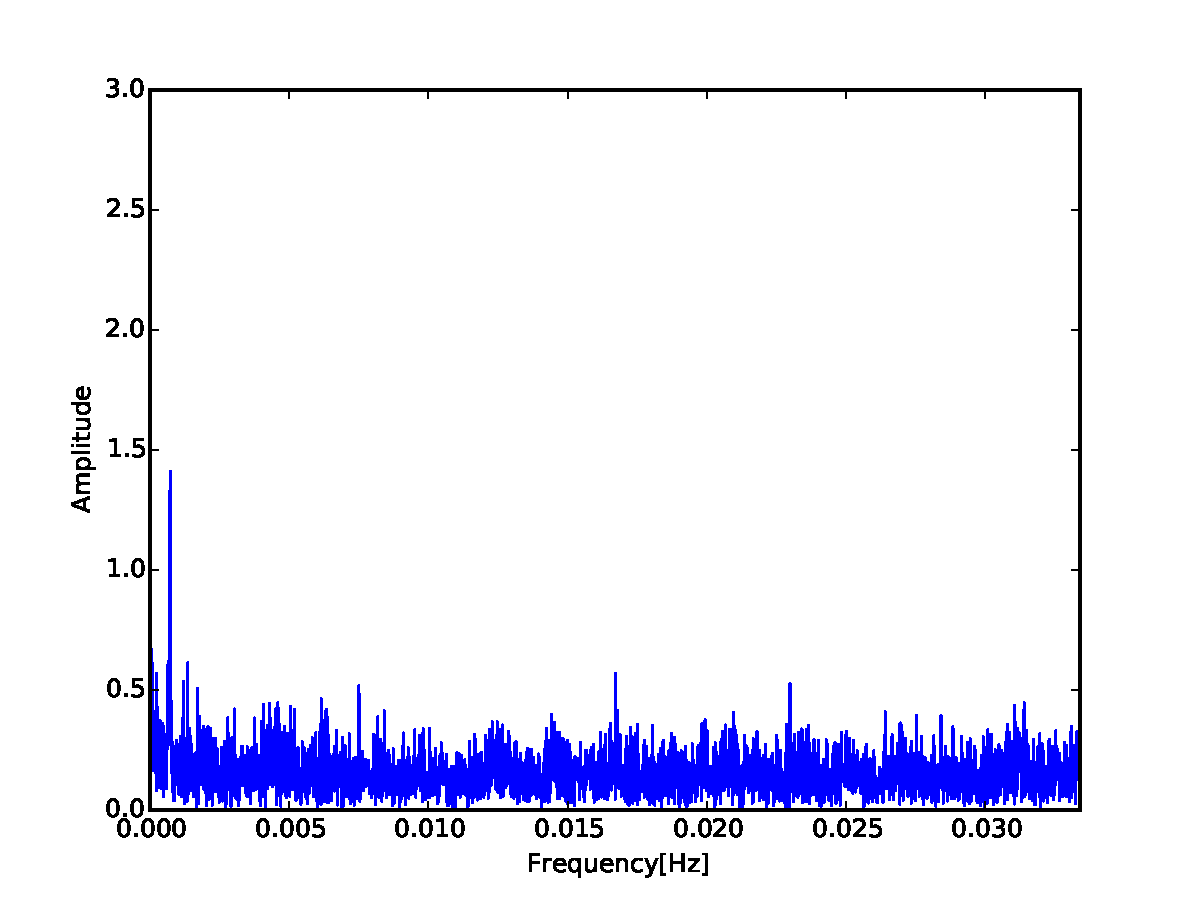
\includegraphics[width=0.33\hsize]{C:/master/mstudy/analysis/long/fft_6-23.pdf}
}~
\subfigure[6 月 24 日]{
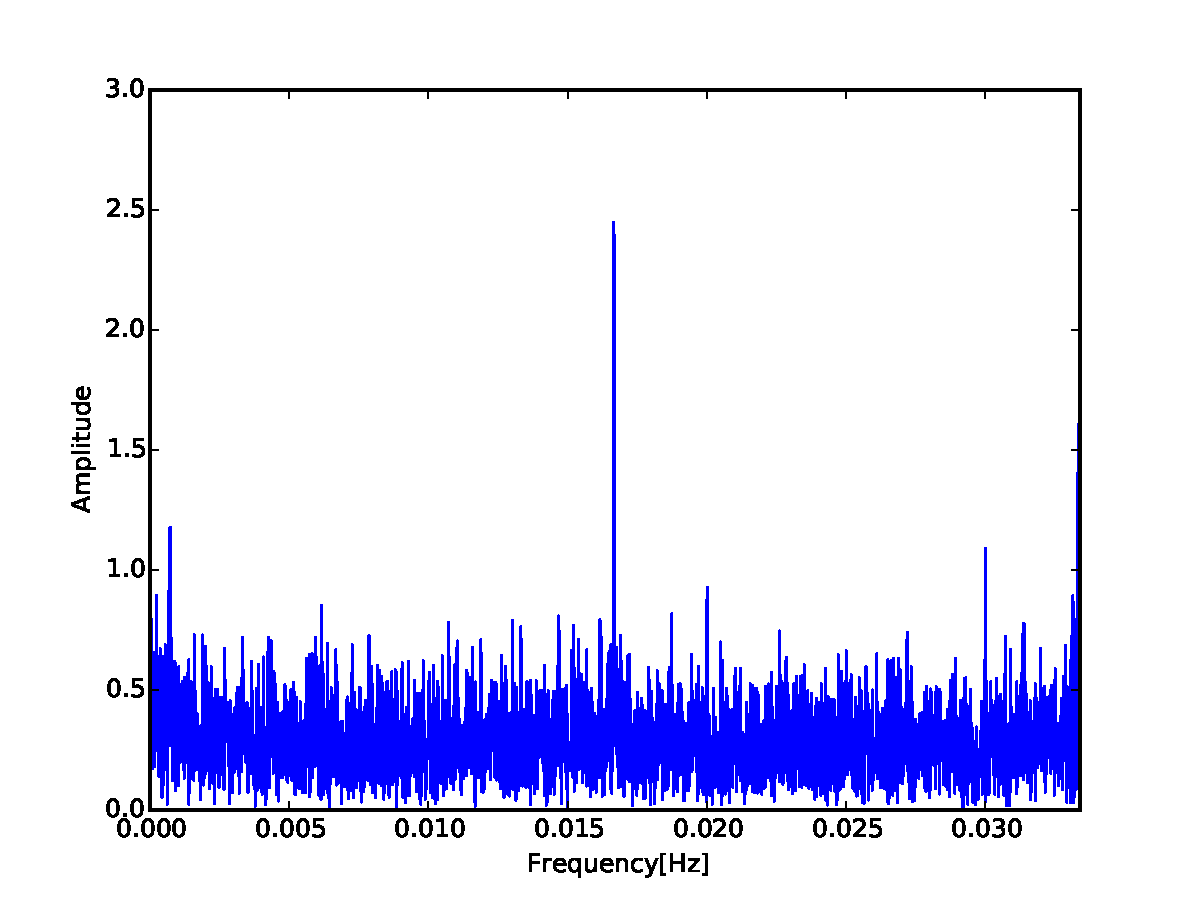
\includegraphics[width=0.33\hsize]{C:/master/mstudy/analysis/long/fft_6-24.pdf}
}~
\subfigure[6 月 25 日]{
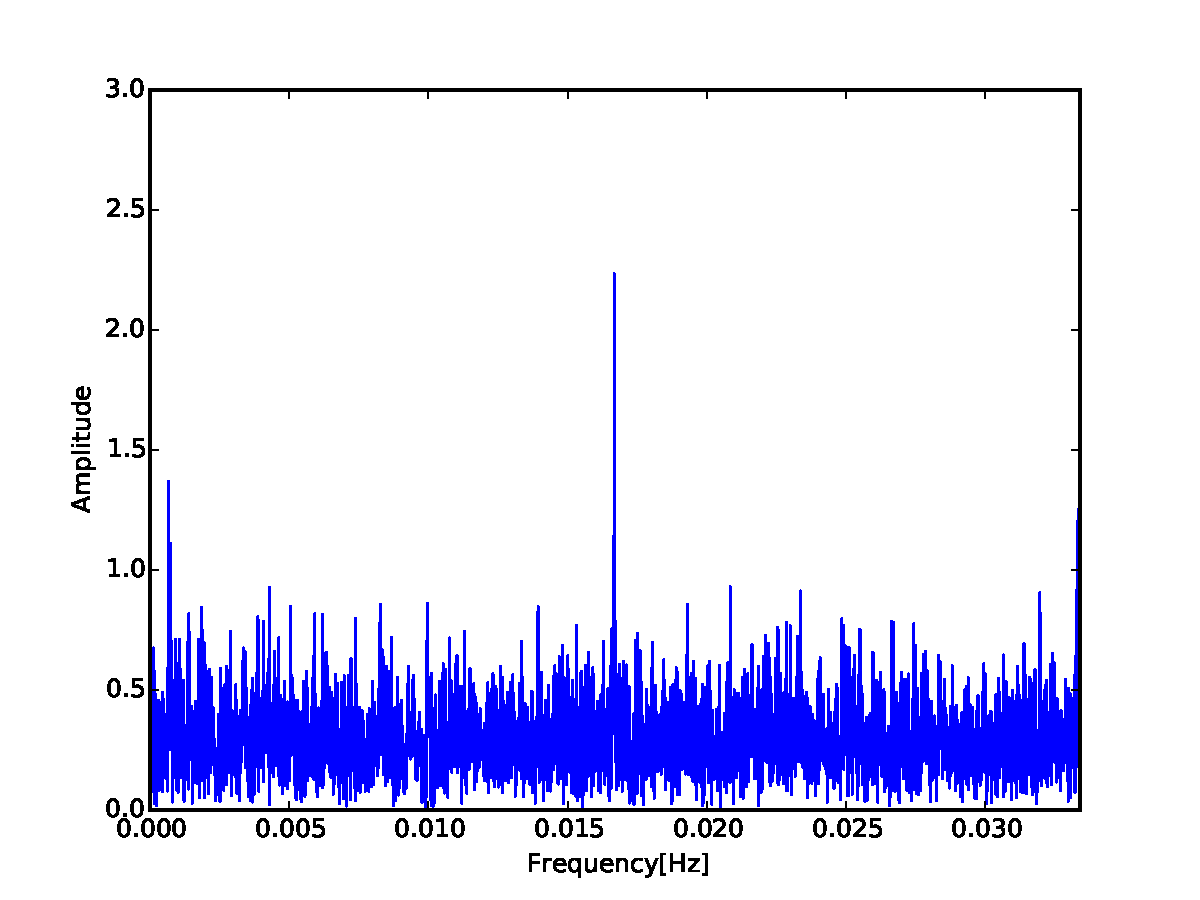
\includegraphics[width=0.33\hsize]{C:/master/mstudy/analysis/long/fft_6-25.pdf}
}
\caption{FFT}
\label{fft}
\end{center}
\end{figure}
図 \ref{fft} より,約 0.0007[Hz](約 24 分)の周波数成分が三つの区間データともに高いことがわかる.計測データの小さな応答遅延の値が時間経過とともに増加する傾向を示す区間の時間的長さは約 30 分程度に見えるため,この周波数成分が知りたい区間の長さに対応すると考えられる.しかしながら一方で,6 月 24 日,6 月 25 日では約 0.017Hz(約 1 分)の周波数成分も大きく出ているため,元データから低遅延帯の波形のみを抽出したよりピンポイントな波形に対する FFT 分析が必要があると考えた.そこで次に,この三つの区間データそれぞれに対し,平均値以下の応答遅延を結んだ波形から移動平均(平滑化パラメータ 0.8)を取った図 \ref{low} の赤線で示す波形に FFT を適用した.その結果を図 \ref{lowfft} に示す.この図から図 \ref{fft} と同様の 0.0007[Hz](約 24 分)の周波数成分が高いことが読み取れる.したがって,低遅延帯が増加傾向を示す長さは 24 分程度であると思われる.
\begin{figure}[tb]
\begin{center}
\subfigure[6 月 23 日]{
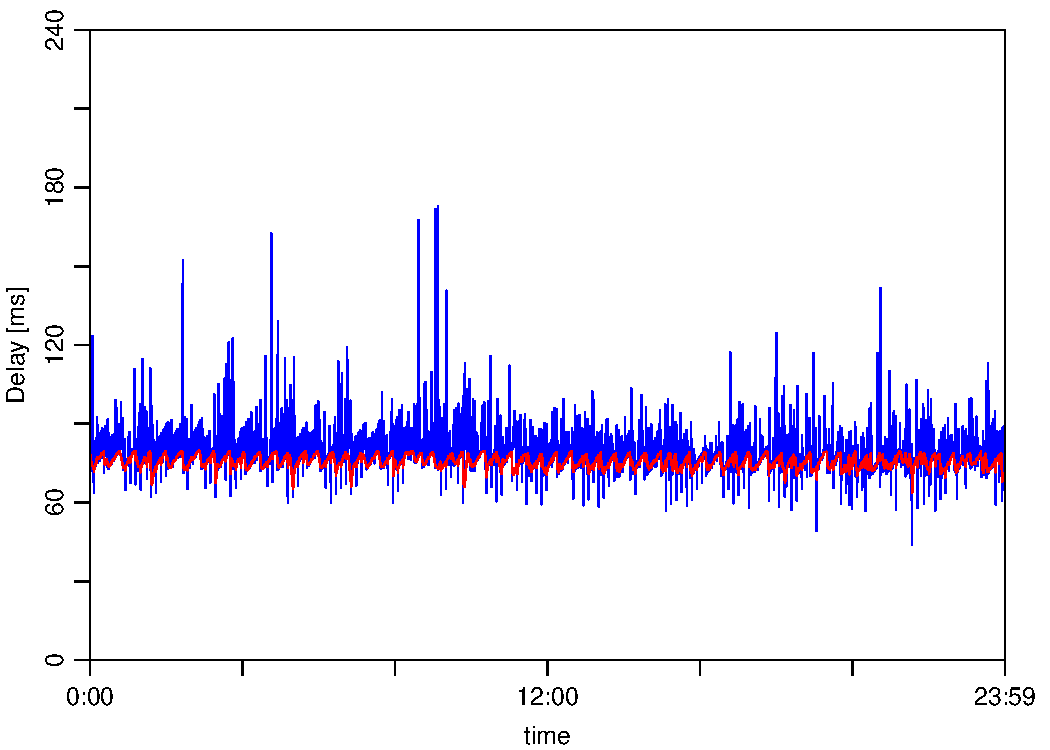
\includegraphics[width=0.5\hsize]{C:/master/mstudy/analysis/long/low_6-23.pdf}
}~
\subfigure[6 月 24 日]{
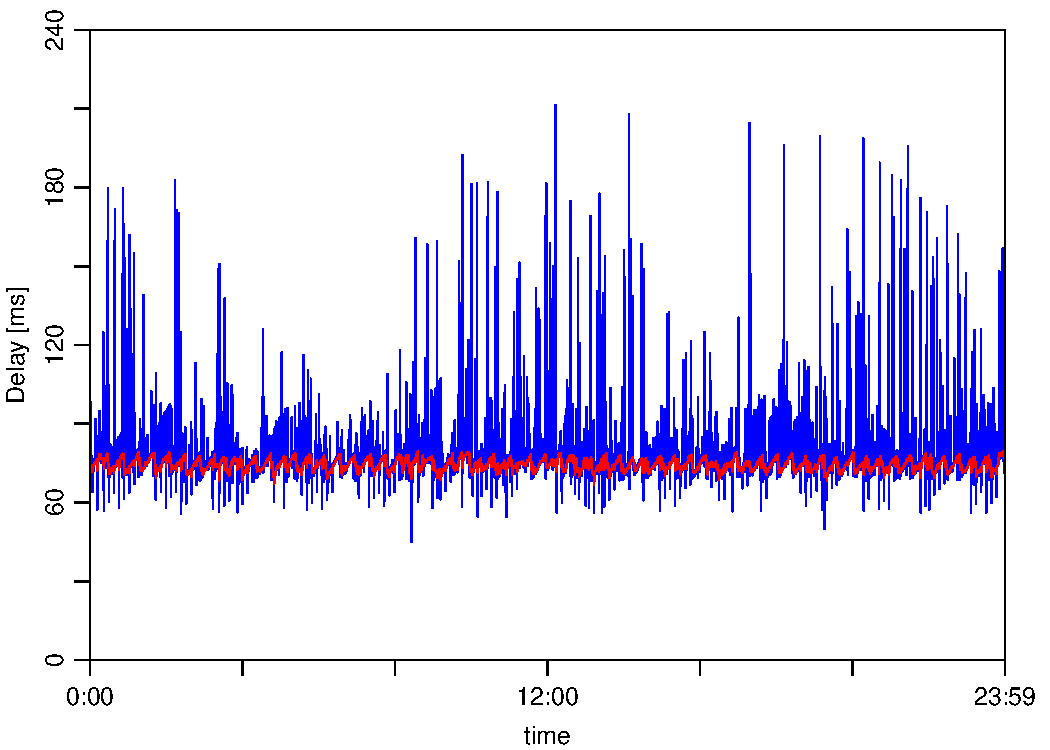
\includegraphics[width=0.5\hsize]{C:/master/mstudy/analysis/long/low_6-24.pdf}
}\\
\subfigure[6 月 25 日]{
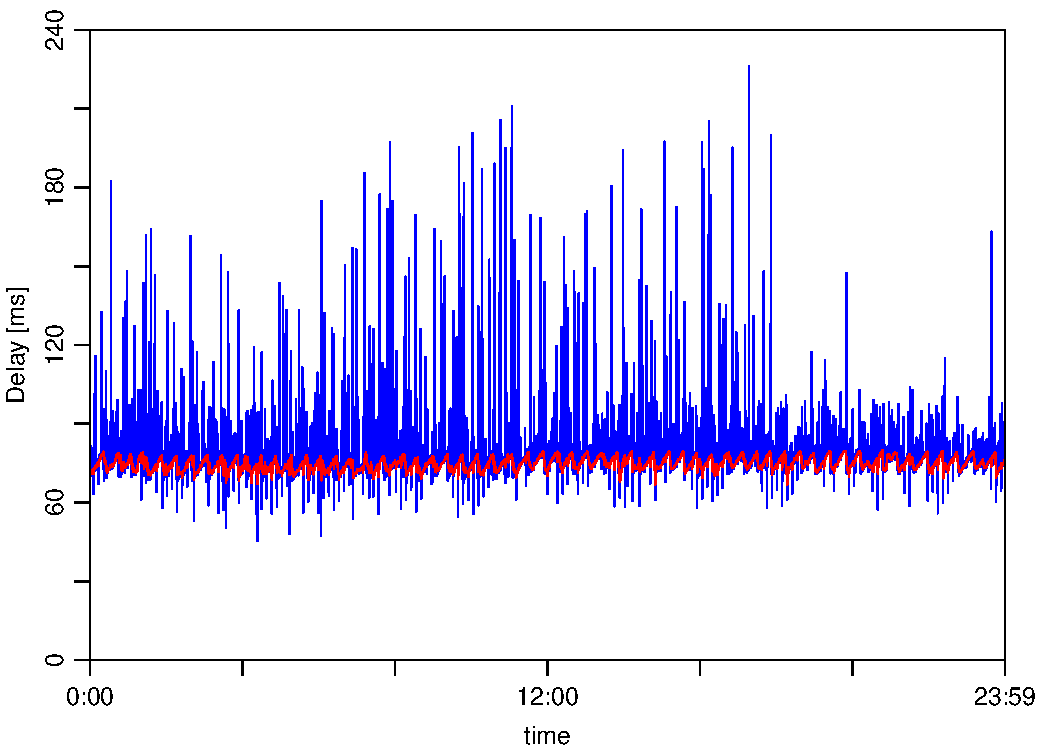
\includegraphics[width=0.5\hsize]{C:/master/mstudy/analysis/long/low_6-25.pdf}
}
\caption{低遅延帯の抽出}
\label{low}
\end{center}
\end{figure}
\begin{figure}[tb]
\begin{center}
\subfigure[6 月 23 日]{
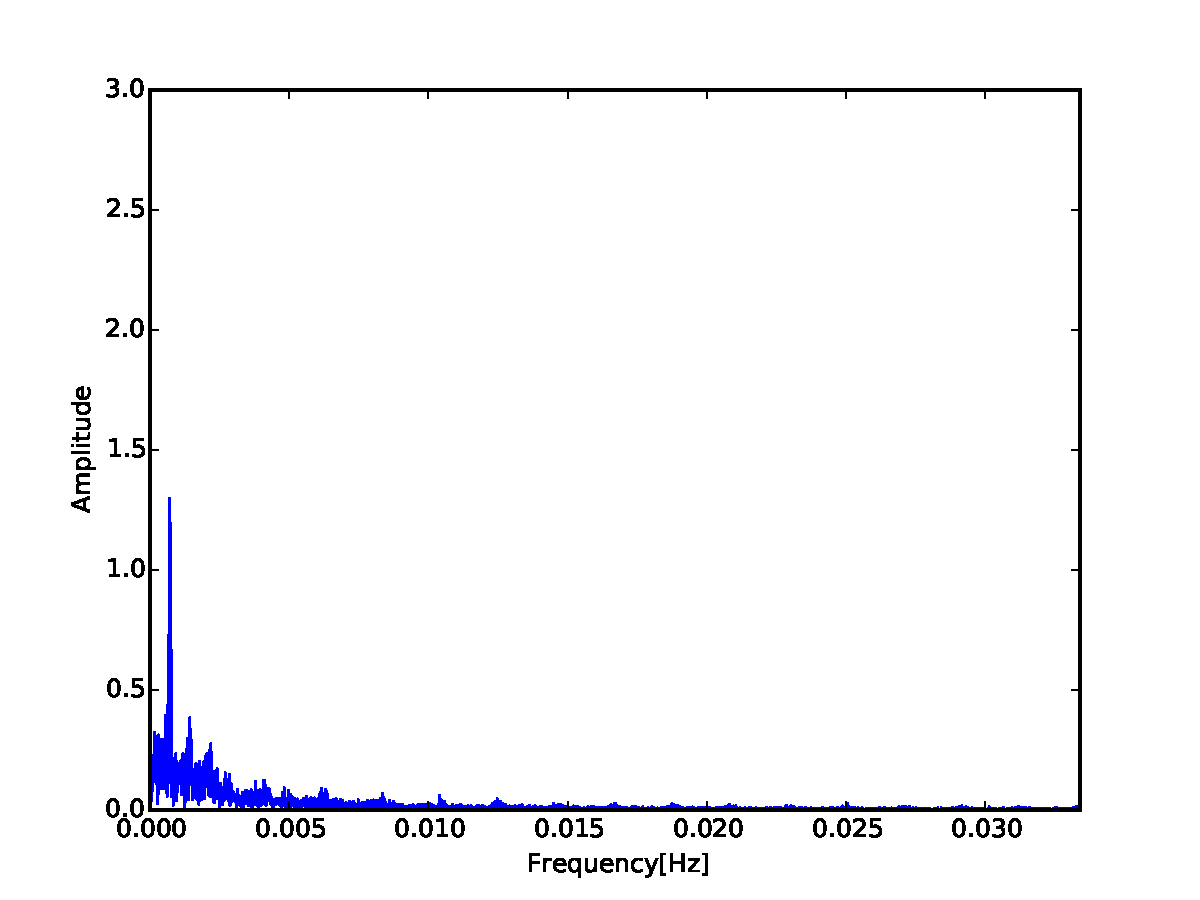
\includegraphics[width=0.33\hsize]{C:/master/mstudy/analysis/long/fft_low_6-23.pdf}
}~
\subfigure[6 月 24 日]{
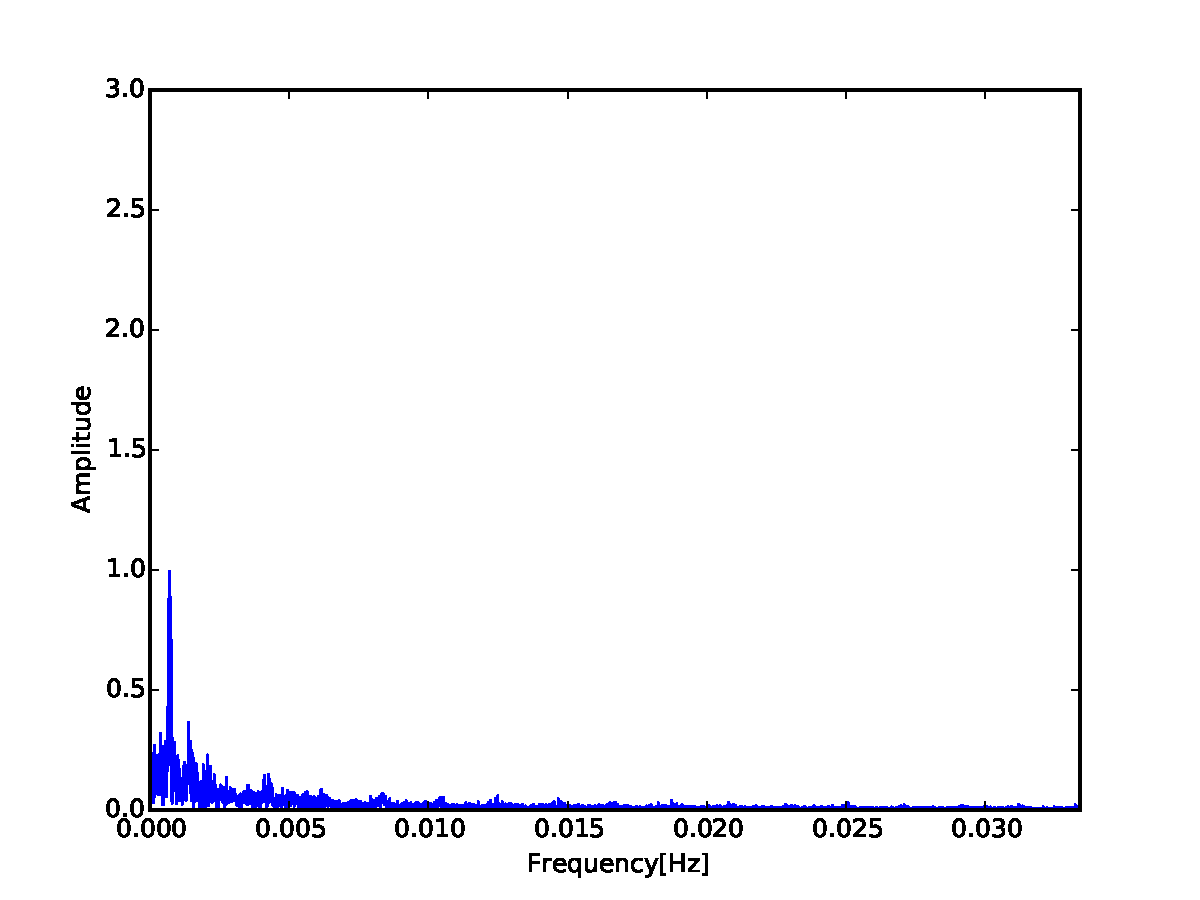
\includegraphics[width=0.33\hsize]{C:/master/mstudy/analysis/long/fft_low_6-24.pdf}
}~
\subfigure[6 月 25 日]{
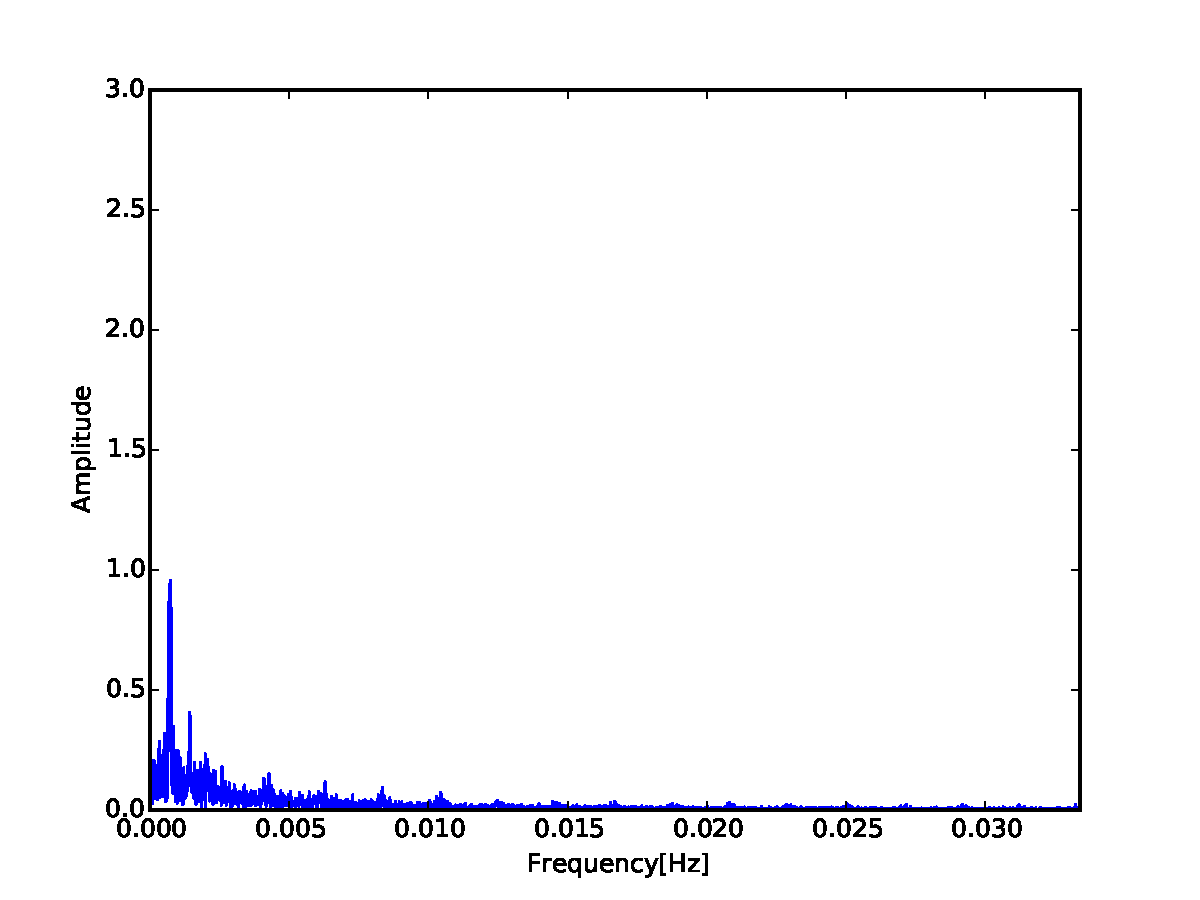
\includegraphics[width=0.33\hsize]{C:/master/mstudy/analysis/long/fft_low_6-25.pdf}
}
\caption{低遅延帯を抽出した波形に FFT を用いた結果}
\label{lowfft}
\end{center}
\end{figure}

\section{のこぎり型の波形の抽出}
一日を通じた計測データでは,応答遅延が緩やかに増加していき,しばらくすると急激に減少して再度緩やかに増加していく傾向がみられる.
ここではこののこぎり型の波形を抽出し各刃の時間的長さを調べることに取り組む.
しかし,応答遅延は短期的な変動が激しく特に突発的に特出して大きなまたは小さな応答遅延が発生するため,のこぎり波の抽出が困難である.
また,平均値以下の応答遅延を直線で結んだ波形から移動平均(平滑化パラメータ 0.8)を取った図 \ref{low} の場合では,のこぎり波形の各両端が滑らかとなり,正確に刃の時間的長さを読み取ることはできなかった.
そこでここでは,ローパスフィルタを用いて短期的な変動を生じさせる高周波数帯を除去した波形をもとに,のこぎり型の波形の抽出に取り組む.

6 月 23 日の 0 時から 15 秒間隔で計測したデータの一部に対してローパスフィルタを用いた結果を図 \ref{lowpass} に示す.
ただし,横軸は計測時刻が早いものから順に 0,1,$\ldots$ としたインデックスを取り,縦軸には応答遅延の値を取っている.
また,青色線が計測値を,黒色線がローパスフィルタを用いて 0.008 [Hz] 以上を除去した波形である.
この 0.008 という値はもと波形の突発的な応答遅延を除去し,かつのこぎり型の波形の各両端が滑らかになりすぎないように試行錯誤のもと定めた.
\begin{figure}[tb]
\begin{center}
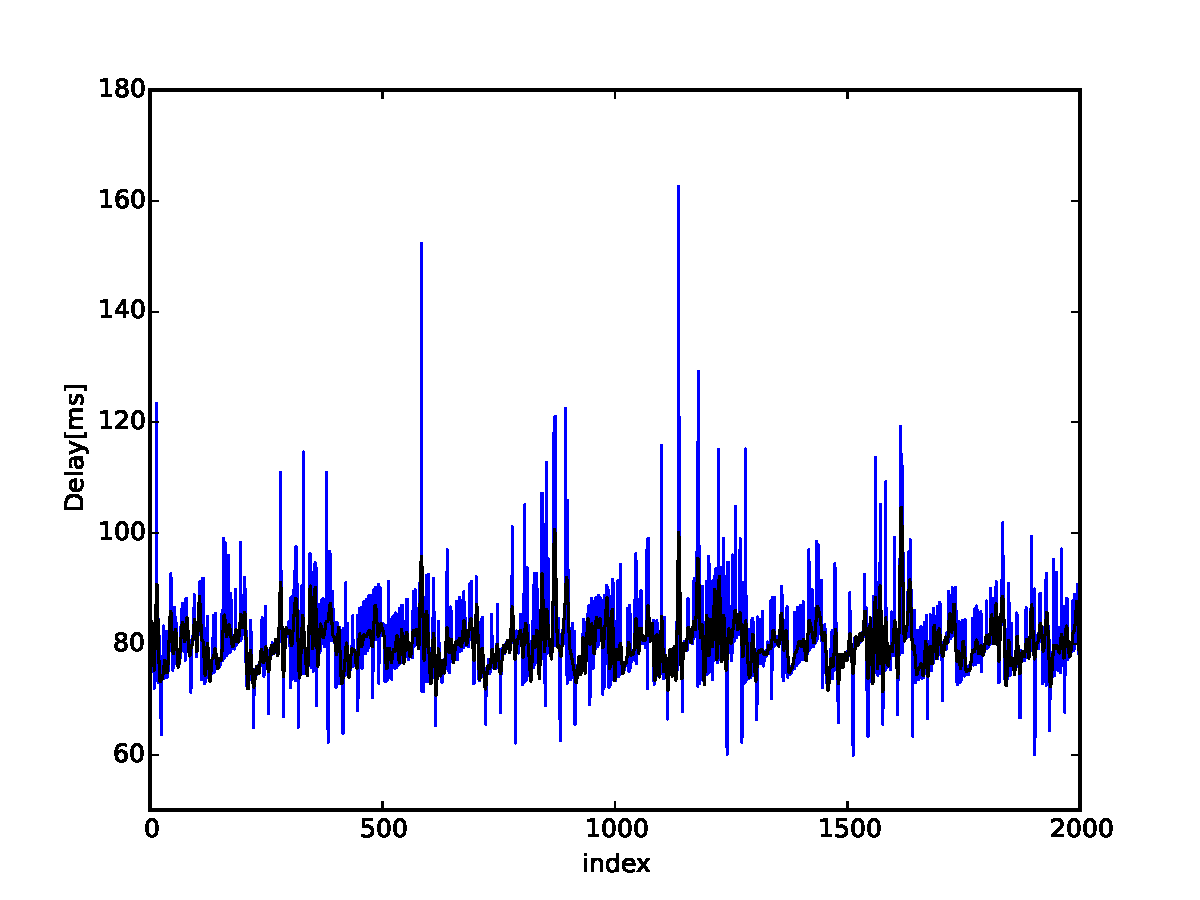
\includegraphics[width=\hsize]{C:/master/mstudy/analysis/long/example1.pdf}
\caption{計測波形(青線)とローパスフィルタを適応した波形(黒線)}
\label{lowpass}
\end{center}
\end{figure}
次にローパスフィルタを適用した波形からのこぎり型の波形を抽出する.

ここでは,波形を右肩上がりの直線で回帰できる区間に分割していく方法を取る.
ただ,全区間を一度に分割することは,分割数がわからないため非常に困難である.
そこで,先頭からインデックス幅 200 (計測時間 50 分相当)の波形を二つに分割し,次に,その分割点からインデックス幅 200 までの波形を二つに分割する操作を繰り返すことで全体を分割する方法を取る.
このインデックス幅 200 (計測時間 50 分相当)は図 \ref{lowfft} からのこぎり型の波形の周期が大体 25 分程度であることをもとに,のこぎり型波形が 2 つよりも多く含まれないように定めた.
また,分割数を 2 つに制約することで,細分化されにくくしようとした.

単回帰には最小二乗法を用い,二つの回帰線の傾きが共に正かつ決定係数の積を最大とする位置で分割した.
以下はこの分割法の疑似コードを示す.\\
\\
$Data <- $計測データの応答遅延値\\
$C <- [0]$ \#分割点(インデックスの集合)\\
\\
$while$\\
$\hspace{0.5cm}for \hspace{0.2cm}i\hspace{0.2cm} in\hspace{0.2cm} [0:200]$\\
\\
$\hspace{1cm}left <- C[末尾]$\\
$\hspace{1cm}mid <- left+i$\\
$\hspace{1cm}right <- left + 200$\\
\\
$\hspace{1cm}Xhead <- [left : mid]$\\
$\hspace{1cm}Yhead <- Data[left : mid]$\\
\\
$\hspace{1cm}Xtail <- [mid : left]$\\
$\hspace{1cm}Ytail <- Data[mid : left]$\\
\\
$\hspace{1cm}\widehat{Y_1} = a_1\widehat{X_2} + b_1 <- 最小二乗法(Xhead,Yhead)$\\
$\hspace{1cm}\widehat{Y_2} = a_2\widehat{X_2} + b_2 <- 最小二乗法(Xtail,Ytail)$\\
\\
$\hspace{1cm}if(a_1>0 \hspace{0.2cm}and \hspace{0.2cm}a_2>0)$\\
$\hspace{1.5cm}C <- C \cup \argmax_{mid} \left[1-\frac{\sum (Yhead - \widehat{Y_1})^2}{\sum (Yhead - \overline{Yhead})^2} \right] * \left[1-\frac{\sum (Ytail - \widehat{Y_2})^2}{\sum (Ytail - \overline{Ytail})^2} \right]$\\
\\
$\hspace{0.5cm}if(mid+200 > データ数)\hspace{1cm}break$\\

結果を図 \ref{result} に示す.
\begin{figure}[tb]
\begin{center}
\subfigure[インデックス 0 から 400 まで(0:00 ~ 1:40 相当)]{
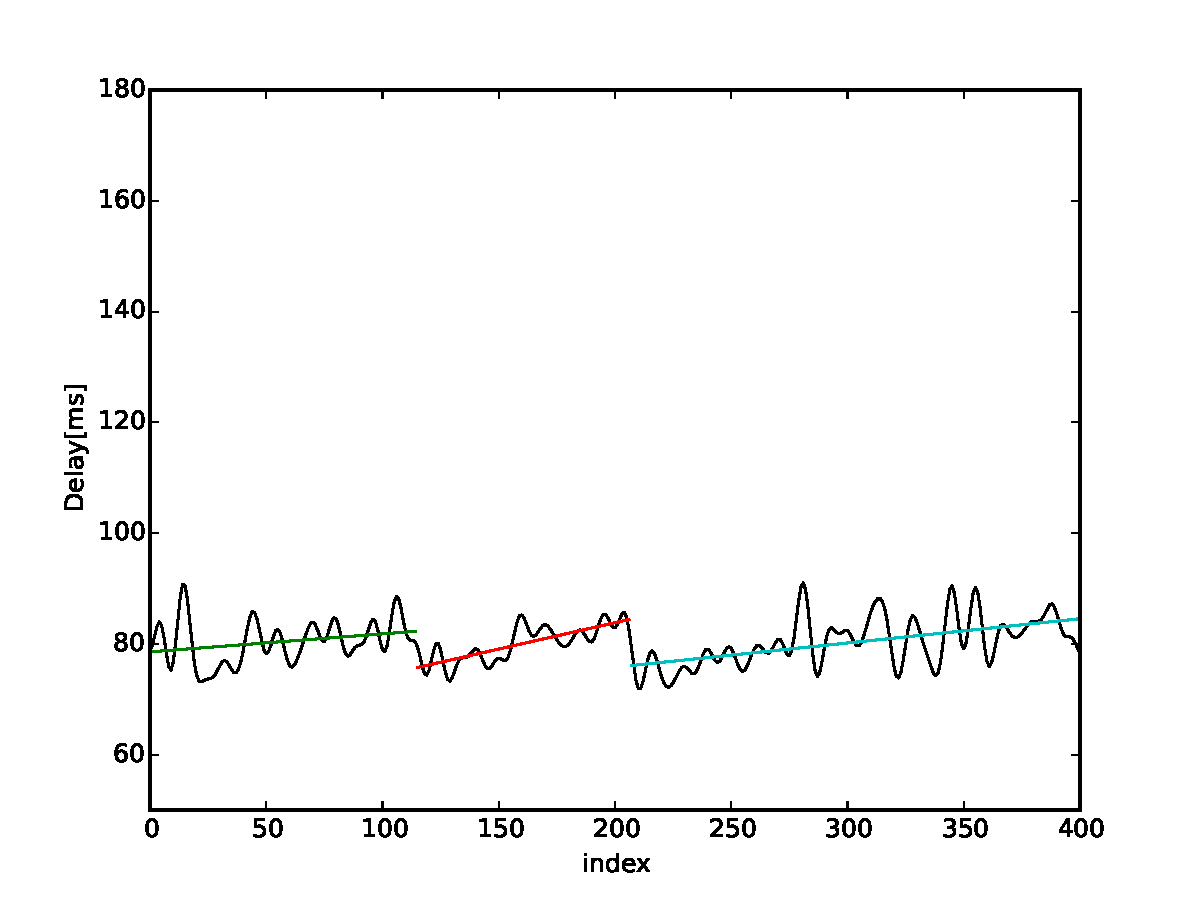
\includegraphics[width=\hsize]{C:/master/mstudy/analysis/long/example2.pdf}
}\\
\subfigure[インデックス 0 から 2000 まで(0:00 ~ 8:20 相当)]{
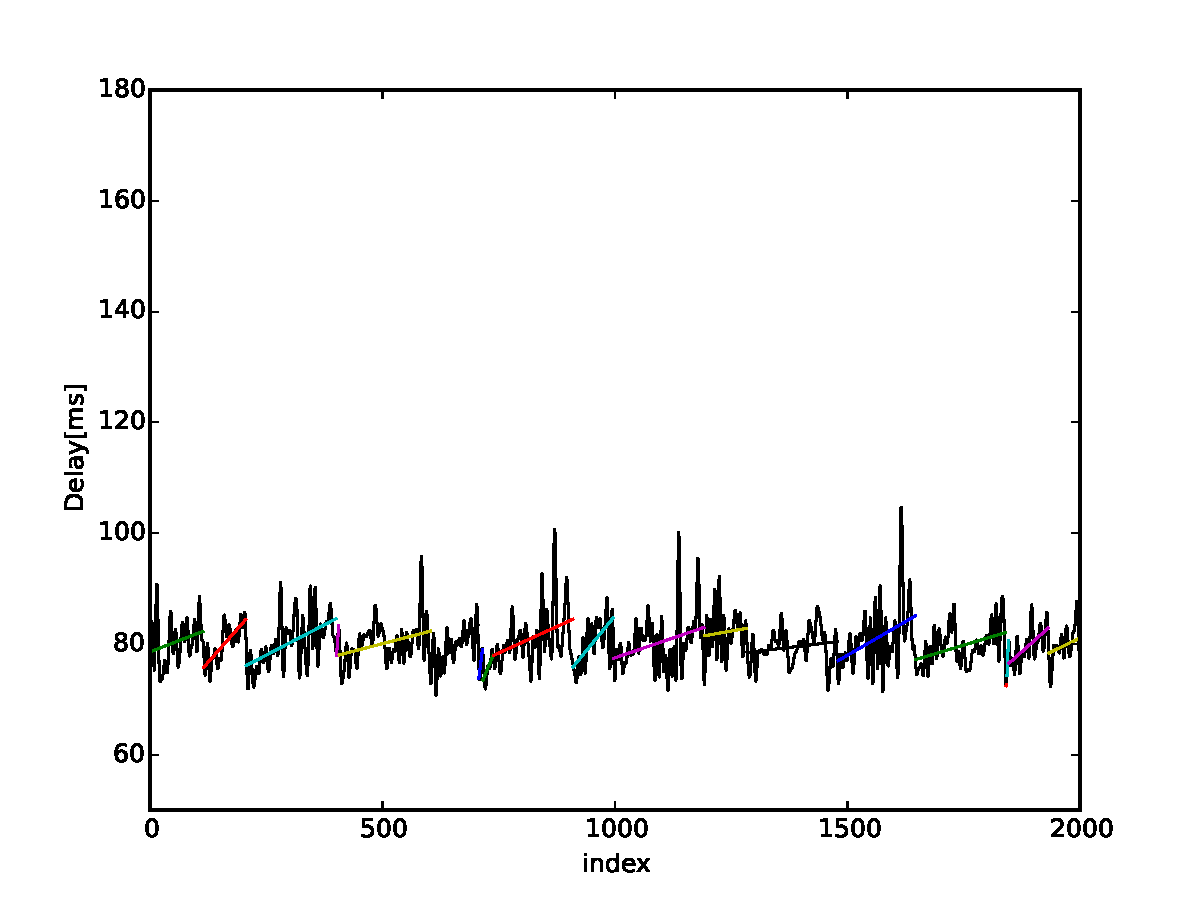
\includegraphics[width=\hsize]{C:/master/mstudy/analysis/long/example3.pdf}
}
\caption{ローパスフィルタ適応後の波形(黒線)と分割により得られる各回帰線}
\label{result}
\end{center}
\end{figure}
図 \ref{result}(a) より,ローパスフィルタ後の波形ではあるが,のこぎり型の波形の両端をほとんどズレなく捉えられていることがわかる.
しかし,図 \ref{result}(b) を見ると,おおよそ期待通りであるが,ごく短い幅で分割されている箇所(インデックス 400 付近の紫線)や逆に分割されていない箇所(インデックス 400 付近から 600 付近にかけての黄色線)が見受けられ,手法の修正が必要である.
短い幅で分割されている箇所に関しては,分割可能な幅の最小値を 20 (5分間相当)などで定めると良いと考える.また, FFT の結果を考慮して定めるとなお良いと思われる.分割されていない箇所に関しては現在検討中である.インデックス幅の最大値を制限することも考えたが,同程度の幅のインデックス 200 から 400 付近の水色線などは十分納得いく分割結果に見えるため,最大値の制限は難しいように感じる.改善点とすれば評価値を決定係数の積ではなく,今回の問題に合わせたものにすることが良いと思われる.
\end{document}